\renewcommand{\figurename}{Rys.}

\chapter{Metodyka pomiaru wysycenia krwi i~częstości akcji serca}
\label{cha:Metodyka}

\fontsize{14}{15}\selectfont
%---------------------------------------------------------------------------

Pulsoksymetria to nowoczesna, nieinwazyjna i~bezbolesna metoda badania tętna i~utlenowania krwi. Oparta na elementarnych prawach fizyki, pozwala 
uzyskać cenne informacje o~układzie krążenia, a~dokładniej - jego zdolności do transportu tlenu w~organizmie. Metoda polega na zasadzie spektrofotometrycznego 
pomiaru wysycenia tlenem hemoglobiny, gdyż hemoglobina utlenowana i~odtlenowana wykazują odmienne właściwości optyczne. Jednocześnie rejestrowana jest również 
częstotliwość pracy serca (tętno).

 
\section{Rola krwi w~procesie wymiany gazowej}
\label{sec:RolaKrwi}

Wymiana gazowa to proces, podczas którego dochodzi do dyfuzji gazów i~ich wymiany między organizmem a~otoczeniem przy pomocy krwi. 
U~człowieka układ krwionośny jest zamknięty~\cite{Fizj:2007}. Znaczy to, że krew nieustannie obiega organizm w~całym systemie połączonych ze sobą 
naczyń krwionośnych. Pompą wymuszającą ten obieg jest serce. Krążenie krwi odbywa się na dwóch drogach: obwodowej oraz płucnej~(rys.~\ref{rys:circ}).

Wymiana gazowa następuje pomiędzy dwoma składnikami atmosfery: tlenem i~dwutlenkiem węgla. W~płucach z~powodu wyższego ciśnienia parcjalnego tlenu 
w~pęcherzykach następuje utlenowanie krwi w~małym obiegu krwi i~dostarczanie jej do tkanek obwodowych.
 
Dostarczany tlen jest niezbędny do zwiększenia wydajności spalania glukozy oraz do tego, by potencjalna energia związków organicznych pochodzących 
z~pokarmu została z~możliwie największą wydajnością zużyta we wszystkich procesach życiowych~\cite{Fizj:2007}.

\begin{figure}[ht]
	\centerline{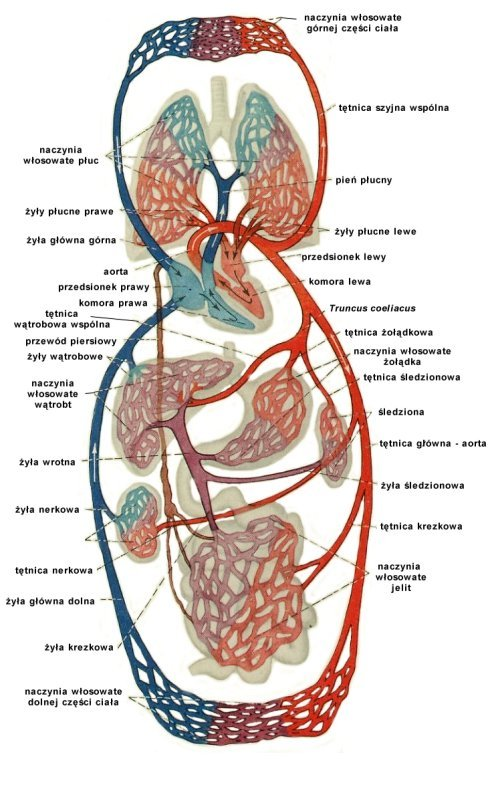
\includegraphics[scale = 0.84]{graphic/obieg_krwi.jpg}}
	\caption{Duży i~mały obieg krwi}
	~\\
	(źródło: http://anatomiac.w.interia.pl)
	\label{rys:circ}
\end{figure}
Krew w~obiegu obwodowym wymienia tlen na dwutlenek węgla w~tkankach organizmu. W~miejscu docelowym krew, poprzez ściany naczyń włosowatych, oddaje tlen 
tkankom o~niższym jego ciśnieniu parcjalnym. Krew częściowo również transportuje dwutlenek węgla~($CO_{2}$), jednak ten jest przenoszony głównie przez 
osocze w~postaci jonowej ($HCO_{3}$)~\cite{Fizj:2007}.
 
\subsection{Skład i~funkcje krwi}
\label{subsec:SkladKrwi}

Krew jest rodzajem tkanki łącznej płynnej. Składa się z~osocza oraz elementów morfotycznych~\cite{Fizj:2007}, których zawartość przedstawia 
tabela~(tab.~\ref{tab:Morfotyczne}).\\

\begin{table}[h]\large
	\caption{Wartości prawidłowe składników morfotycznych i~chemicznych we krwi~\cite{SzGa11}}
	\label{tab:Morfotyczne}
	\begin{center}
	\begin{tabular}{|c||c|c|}
	\hline
	Składnik & \multicolumn{2}{|c|}{Normy}	\\
	\hline \hline

	\multirow{2}{*}{Erytrocyty (RBC)} & \multicolumn{2}{|c|}{$4,2 - 5,4~ mln/mm^3$ (M)} \\
	\cline{2-3} & \multicolumn{2}{|c|}{$3,4 - 5,2~mln/mm^3$ (K)} \\ 
	\hline	

	Leukocyty (WBC) & \multicolumn{2}{|c|}{$4 - 7~tys/mm^3$} \\
	\hline

	Trombocyty (PLT) & \multicolumn{2}{|c|}{$150 - 300~tys/mm^3$} \\
	\hline
	\multirow{2}{*}{Hematokryt (HC)} & \multicolumn{2}{|c|}{$42\% - 52\%$ (M)} \\
	\cline{2-3} & \multicolumn{2}{|c|}{$37\% - 47\%$ (K)} \\
	\hline

	MCHC  & \multicolumn{2}{|c|}{$32 - 36~g/100 ml$}\\
	\hline
	\multirow{2}{*}{Hemoglobina} & \multicolumn{2}{|c|}{$14 - 18~g/dl$ (M)} \\ 
	\cline{2-3} & \multicolumn{2}{|c|}{$12 - 16~g/dl$ (K)} \\ 
	\hline

	Karboksyhemoglobina & \multicolumn{2}{|c|}{do 3\% hemoglobiny} \\
	\hline
	\end{tabular}
	\end{center}
	~\\
	(źródło: Na podstawie \cite{SzGa11})
\end{table}
Osocze krwi stanowi płynną część krwi, stanowiącą 4,5\% ciężaru ciała, w~której zawieszone są elementy morfotyczne~(rys.~\ref{rys:osocze}).
Składa się głównie z~wody (92\%) i~rozpuszczonych w~niej białek osocza: albumin, globulin, fibrynogenu i~innych czynników krzepnięcia (zarówno aktywujących, jak 
i~hamujących ten proces), ciał tłuszczowych, glukozy, elektrolitów i~wielu innych składników organicznych i~nieorganicznych~\cite{Fizj:2007}.

\begin{figure}[!ht]
	\centerline{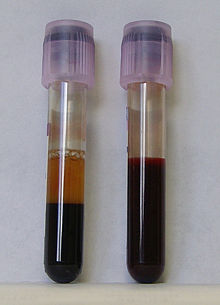
\includegraphics[scale = 0.64]{graphic/osocze.jpg}}
	\caption{Próbki krwi. Po prawej krew świeżo pobrana, po lewej krew z~substancją zapobiegającą krzepnięciu. Widoczne jaśniejsze osocze, pod 
		 którym osadziły się składniki komórkowe}
	~\\
	(źródło: Na podstawie \cite{Dwyer:2008})
	\label{rys:osocze}
\end{figure}
\noindent Transport atomów tlenu przez krew w~ustroju jest możliwa dzięki cząsteczkom hemoglobiny zawartej w~krwinkach czerwonych. 
Hemoglobina ($Hb$) jest białkiem, składającym się z~czterech łańcuchów polipeptydowych~\cite{Fizj:2007}, z~których każdy łączy się w~płucach 
z~jedną cząsteczką~$0_{2}$~(rys.~\ref{rys:hemoglobina}). 
\begin{figure}[!ht]
\centerline{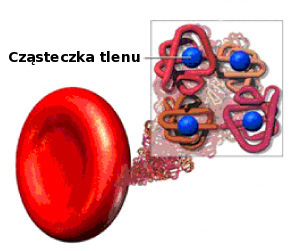
\includegraphics[scale = 0.66]{graphic/hemoglobina.jpg}}
	\caption{Cząsteczki hemoglobiny zawarte w~erytrocytach umożliwiają wiązanie oraz transport cząsteczek tlenu}
	\label{rys:hemoglobina}
	~\\
	(źródło: Na podstawie \cite{Dwyer:2008})
\end{figure}

\noindent Nietrwałe połączenie cząsteczek tlenu z~cząsteczką hemoglobiny tworzy oksyhemoglobinę~($HbO_{2}$).

\subsection{Saturacja $SaO_{2}$ a~$SpO_{2}$}
\label{subsec:Saturacja}

Hemoglobina ($Hb$) wykazuje zdolność do wiązania z~wieloma pierwiastkami oraz związkami chemicznymi tworząc trwałe lub nietrwałe połączenia. 
Oksyhemoglobina ($HbO_{2}$), karboksyhemoglobina ($HbCO$), sulfohemoglobina ($SulfHb$) oraz methemoglobina ($MetHb$) to najistotniejsze związki 
z~punktu widzenia efektywności transportu tlenu. 

W~diagnostyce medycznej rozróżnia się dwa wskaźniki wysycenia krwi: $SpO_{2}$ oraz $SaO_{2}$. 
Parametr $SaO_{2}$ definiowany jako procentowa zawartość oksyhemoglobiny w~całkowitej ilości hemoglobiny~(\ref{equ:SaO2}), 
wyznaczany jest metodą inwazyjną opartą o~analizę chemiczną pobranej próbki krwi~(in~vitro).

\begin{equation}
\label{equ:SaO2}
	SaO_{2} = \frac{HbO_{2}}{HbO_{2} + Hb + HbCO + metHb + SulfHb} * 100\%
\end{equation}

Inwazyjna metoda wyznaczania saturacji $SaO_{2}$ pozwala na określenie poprawnej zawartości hemoglobiny utlenowanej, bez uwzględnienia hemoglobiny 
dysfunkcyjnej. Istnienie wielu rodzajów dyshemoglobiny niezdolnej do prawidłowego transportu tlenu, jak $metHb$ oraz $HbCO$ wprowadza błędy pomiarowe
nasycenia krwi przy pomiarach metodami optycznymi. Metody pomiaru saturacji częściowej $SpO_{2}$ oparte o~analizę stopnia absorpcji promieniowania 
przez składniki krwi nie odróżniają odmian hemoglobiny połączonej ze związkami tlenu~\cite{Fizj:2007}. Skutkiem niedoskonałości metod optycznych jest
zawyżanie wartości nasycenia w~przypadku występowania hemoglobiny dysfunkcyjnej~(\ref{equ:SpO2}). 

\begin{equation}
\label{equ:SpO2}
	SpO_{2} = \frac{HbO_{2} + HbCO + metHb}{HbO_{2} + Hb + HbCO + metHb + SulfHb} * 100\%
\end{equation}
\\
\noindent Podczas zatrucia tlenkiem węgla, którego powinowactwo do hemoglobiny jest 250-300 razy większe niż tlenu, wskaźnik nasycenia $SpO_{2}$ 
osiąga wartość 100\%, mimo braku zdolności do prawidłowego transportu tlenu. 

\section{Spektrofotometria 'in vivo'}
\label{sec:InVivo}

Spektroskopia absorpcyjna i~odbiciowa w~bliskim nadfiolecie, świetle widzialnym oraz w~podczerwieni znajdują szerokie zastosowanie w~chemii analitycznej, 
biologii, medycynie i~badaniach materiałowych.
Selektywna absorpcja zespołów komórek umożliwia wykorzystanie w~diagnostyce medycznej zasad i~praw spektrofotometrii. Zdecydowana większość analiz 
medycznych przeprowadzanych jest przy wykorzystaniu zasad fotometrii, a~z~tego aż około 90\% opiera się na zasadach spektrofotometrii. Oznacza 
się w~ten sposób poziom hormonów, przeprowadza testy enzymatyczne, bada kinetykę reakcji chemicznych~\cite{Cys:2007}. 

Badania spektofotometryczne przeprowadzane są w~układzie łącza optycznego: źródło promieniowania, kuweta pomiarowa, odbiornik promieniowania.
Spektrofotometria 'in vivo' jest badaniem laboratoryjnym przeprowadzanym na organizmie żywym bez konieczności pozyskiwania próbek metodami inwazyjnymi.

\subsection{Okno optyczne tkanek}
\label{subsec:OknoOptyczne}

Badany obiekt biologiczny~(rys.~\ref{rys:finger}) składa się z~ciał stałych, cieczy i~gazów absorbujących promieniowanie świetlne, 
charakteryzujących się indywidualnym widmem absorpcyjnym~\cite{Nui:2007}. Woda, związki hemoglobiny, lipidy, melanina, mioglobina, 
cytochromy, bilirubina oraz karotenoidy to podstawowe chromofory ustroju~\cite{Haggblad:2008}. 

\begin{figure}[ht]
\centerline{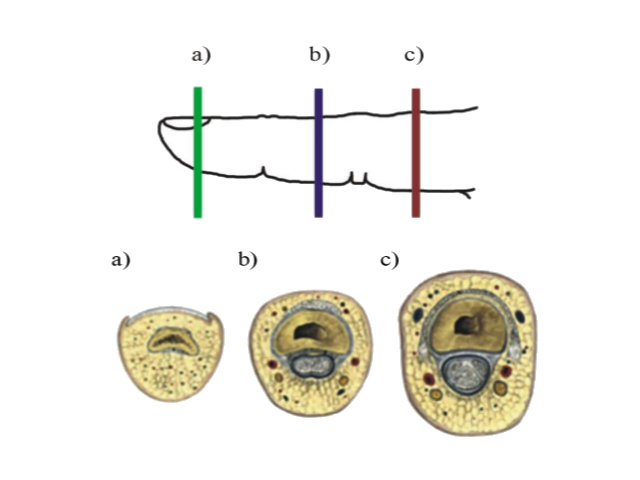
\includegraphics[scale = 0.56]{graphic/finger.png}}
	\caption{Kolejne przekroje tkanek palca ludzkiego}
	\label{rys:finger}
	~\\
	(źródło: Na podstawie \cite{Cys:2007})
\end{figure}

Równanie~(\ref{equ:multilayer2}) przedstawia całkowity współczynnik absorpcji niejednorodnej mieszaniny związków, który jest równy sumie ich indywidualnych 
współczynników pochłaniania.

Celem zwiększenia skuteczności pomiaru absorpcji użytecznego promieniowania świetlnego przez składniki krwi, należy zminimalizować wpływ pochłaniania użytecznego
promieniowania przez pozostałe chromofory środka. Odmienne widma absorpcyjne związków pochłaniających zmuszają do obrania optymalnego zakresu promieniowania
świetlnego.

\subsubsection{Woda}
\label{subsubsec:Woda}

Woda stanowi od 60\% do 80\% całkowitej masy ciała i~jest głównym składnikiem płynów ustroju, m.in.~krwi i~limfy. Z~powodu wysokiej koncentracji, $H_{2}O$ 
w~większości tkanek biologicznych jest najistotniejszym medium absorbującym w~pomiarach spektroskopowych. Widmo absorpcyjne wody w~zakresie 200~-~10000~nm 
oraz 650~-~1050~nm przedstawia rysunek \ref{rys:water}.

\begin{figure}[ht]
\centerline{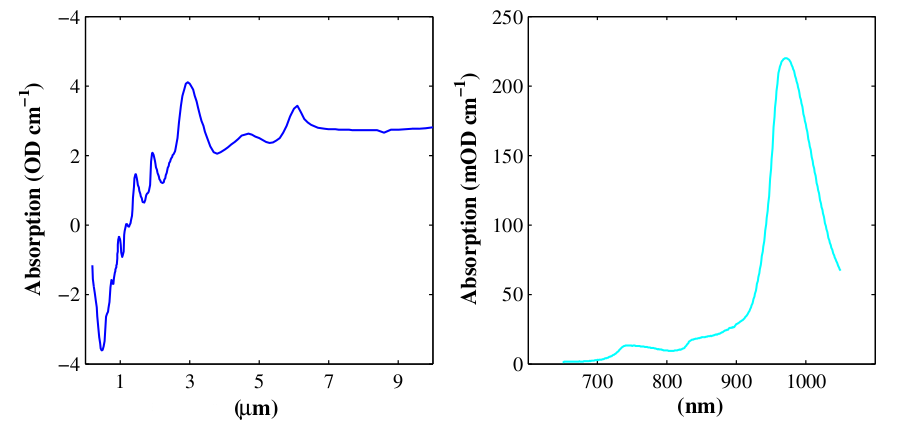
\includegraphics[scale = 0.56]{graphic/water.png}}
	\caption{Widmo absorpcyjne czystej wody}
	\label{rys:water}
	~\\
	(źródło: Na podstawie \cite{Haggblad:2008})
\end{figure}
\noindent W~obszarze 200~-~900 nm istnieje przedział stosunkowo niskiej absorpcji promieniowania. Powyżej granicy 900 nm współczynnik pochłaniania gwałtownie 
wzrasta, skutecznie pochłaniając promieniowanie z~tego zakresu długości fali.

\subsubsection{Związki hemoglobiny}
\label{subsubsec:hemoglobina}

Zdolność hemoglobiny do absorpcji promieniowania świetlnego silnie zależy od zawartości tlenu. Hemoglobina bogata w~cząsteczki $O_{2}$ (oksyhemoglobina) 
wykazuje lokalne maksima pochłaniania dla długości fali w~zakresie 576~-~542 nm oraz globalne maksimum dla 415~nm. Widmo absorpcyjne deoksyhemoglobiny 
posiada lokalne maksima pochłaniania dla 420~nm, 555~nm oraz 756~nm~(rys.~\ref{rys:hb}). Dla promieniowania o~długości fali do 560~nm współczynniki absorpcji 
oksyhemoglobiny oraz deoksyhemoglobiny są zbliżone.  
\begin{figure}[!ht]
\centerline{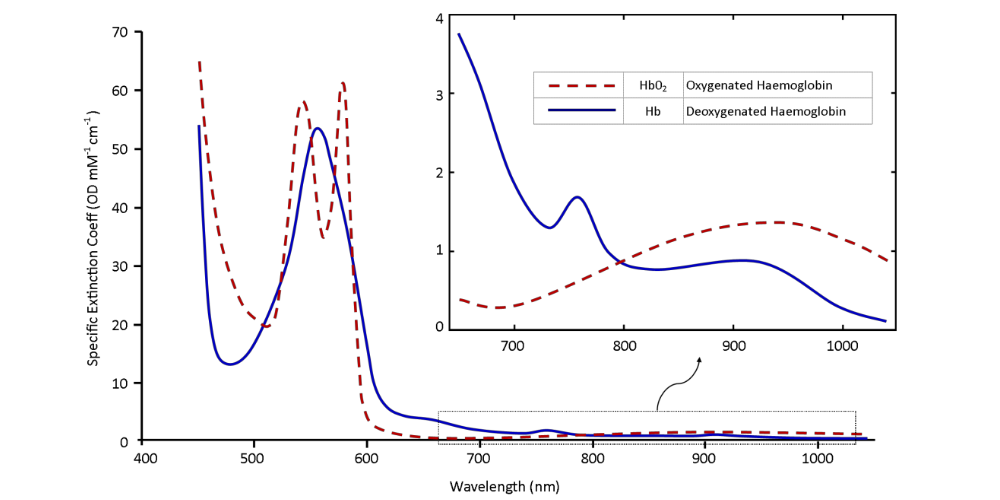
\includegraphics[scale = 0.54]{graphic/hb.png}}
	\caption{Widmo absorpcyjne deoksyhemoglobiny i~oksyhemoglobiny. Charakterystyczny punkt izozbestyczny dla 800 nm}
	\label{rys:hb}
	~\\
	(źródło: Na podstawie \cite{Haggblad:2008})
\end{figure}

\noindent Istotnym obszarem z~punktu widzenia spektrofotometrii jest zakres promieniowania od 600~nm do 1000~nm, gdzie związki hemoglobiny wykazują odrębne właściwości 
optyczne~(rys.~\ref{rys:blood}). Dla długości fali około 800~nm istnieje punkt izozbestyczny, w~którym absorpcja dla obu rodzajów hemoglobiny jest identyczna.
\subsubsection{Mioglobina}
\label{subsubsec:hemoglobina}

Jest to białko zbliżone budową do hemoglobiny, służące do magazynowania tlenu w~mięśniach czerwonych (poprzecznie prążkowanych)~\cite{Haggblad:2008}. 
Wyróżnia się deoksymioglobinę, oksymioglobinę, karboksymioglobinę oraz metmioglobinę. Rysunek~\ref{rys:mioglobin} przedstawia widmo absorpcyjne 
związków mioglobiny.
\begin{figure}[h]
\centerline{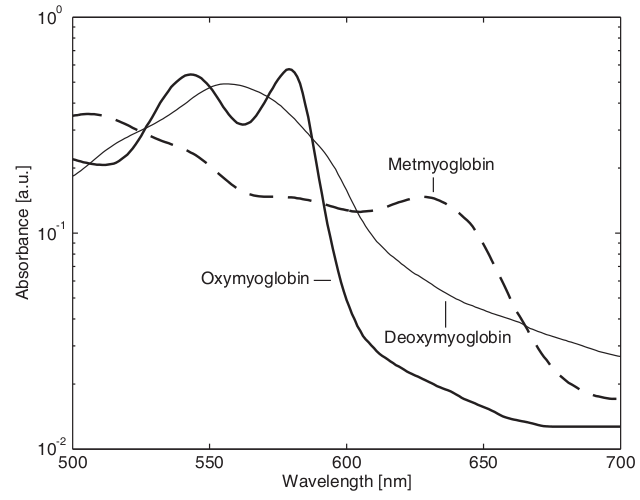
\includegraphics[scale = 0.50]{graphic/mioglobin.png}}
	\caption{Widmo absorpcyjne deoksymioglobiny, oksymioglobiny oraz metmioglobiny}
	\label{rys:mioglobin}
	~\\
	(źródło: Na podstawie \cite{Haggblad:2008})
\end{figure}

\subsubsection{Melanina}
\label{subsubsec:melanina}

Melanina to pigment występujący w~skórze właściwej, naskórku, włosach oraz w~tęczówce oka, odpowiedzialny za ich barwę. Melaniny w~skórze chronią jej 
głębsze warstwy przed szkodliwym promieniowaniem ultrafioletowym UV zawartym w~promieniowaniu słonecznym. Pod wpływem promieni słonecznych ilość melaniny 
zwiększa się, powodując przejściową zmianę zabarwienia skóry~\cite{Haggblad:2008}. Wśród melanin wyróżnia się m.in. eumelaninę, feomelaninę i~neuromelaninę. 
Eumelanina jest barwnikiem czarnobrązowym, feomelanina jest pigmentem o~zabarwieniu żółtoczerwonym.
\begin{figure}[h]
\centerline{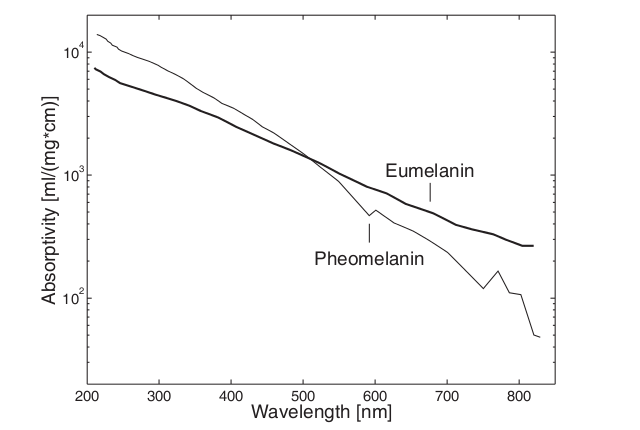
\includegraphics[scale = 0.55]{graphic/melanin.png}}
	\caption{Widmo absorpcyjne eumelaniny oraz feomelaniny}
	\label{rys:melanin}
	~\\
	(źródło: Na podstawie \cite{Haggblad:2008})
\end{figure}

\subsubsection{Inne chromofory}
\label{subsubsec:hromofory}

Łączna ilość endogennych związków absorbujących, znajdujących się w~tkankach żywych jest ogromna. Jednak większość z~nich jest obecnych tylko
w~mniejszych stężeniach, co czyni je mniej znaczącymi. Inne są aktywne w~regionach długości fali spoza zakresu fal promieniowania widzialnego i~bliskiej podczerwieni.

\subsubsection{Spektrofotometria w~bliskiej podczerwieni (NIR)}
\label{subsubsec:NIR}

Niejednorodny zbiór żywych tkanek wykazuje w~analizie spektralnej okno optyczne~(rys.~\ref{rys:window}), w~którym przenikanie promieniowania w~głąb organizmu jest maksymalne. 
Zdolność wody do przepuszczania promieniowania widzialnego i~bliskiej podczerwieni (650~-~1050~nm) umożliwia skuteczną realizację nieinwazyjnej transluminacji takiego zbioru 
tkanek żywych~\cite{Cys:2007}. 
\begin{figure}[ht]
\centerline{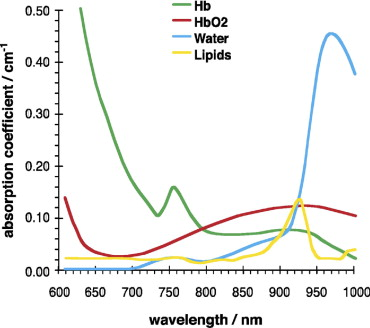
\includegraphics[scale = 1.20]{graphic/window.jpg}}
	\caption{Widma absorpcyjne podstawowych chromoforów tkanek żywych. Charakterystyczne okno optyczne w~zakresie długości fali 650~-~1050~nm}
	\label{rys:window}
	~\\
	(źródło: Na podstawie \cite{Haggblad:2008})
\end{figure}

\subsection{Transluminacja a~metoda refleksyjna}
\label{subsec:TransReflex}

Podczas przeprowadzania procesu prześwietlania lub podświetlania tkanek, szczególnie wówczas, gdy badanie jest długotrwałe, konieczne jest właściwe pozycjonowanie obiektu badanego 
względem układu pomiarowego. Unieruchomienie nie może wpłynąć na stan funkcjonalny badanego ośrodka przy jednoczesnym zachowaniu komfortu. Typowe sposoby pozycjonowania układu 
pomiarowego w~postaci źródeł promieniowania i~detektorów przedstawia rysunek~\ref{rys:position}. 

Przeprowadzanie badań diagnostycznych metodą transluminacji oparte jest o~akwizycję sygnału świetlnego po przejściu przez badany ośrodek, przy ustawieniu detektora 
po przeciwnej stronie obiektu~(rys.~\ref{rys:position}~a). Odebrane promieniowanie optyczne staje się nośnikiem informacji o~charakterystycznych parametrach dotyczących 
właściwości tego obiektu. Diagnostyka spektrofotometryczna przy pomocy metody refleksyjnej możliwa jest dzięki występowaniu rozpraszania wstecznego promieniowania 
świetlnego w~badanym obiekcie biologicznym~\ref{rys:redlight}~b. Promieniowanie w~ośrodku ulega załamaniu, absorpcji oraz wielokrotnemu rozproszeniu, następnie zostaje 
pochłonięte w~detektorze poza ośrodkiem~(rys.~\ref{rys:position}~b,~c). 
\begin{figure}[!ht]
\centerline{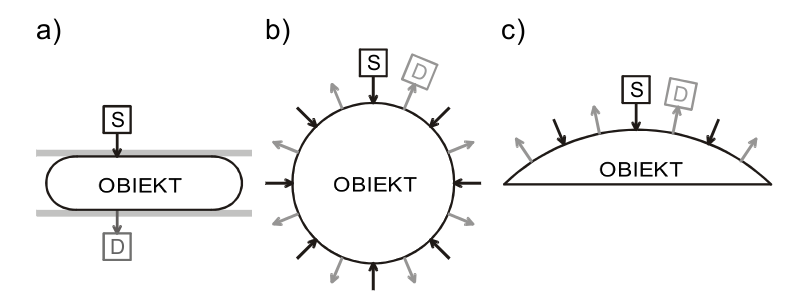
\includegraphics[scale = 0.50]{graphic/position.png}}
	\caption{Metody pozycjonowania badanego obiektu względem układu pomiarowego, S - źródło promieniowania, D - detektor promieniowania}
	\label{rys:position}
	~\\
	(źródło: Na podstawie \cite{Cys:2007})
\end{figure}
\begin{figure}[!ht]
\centerline{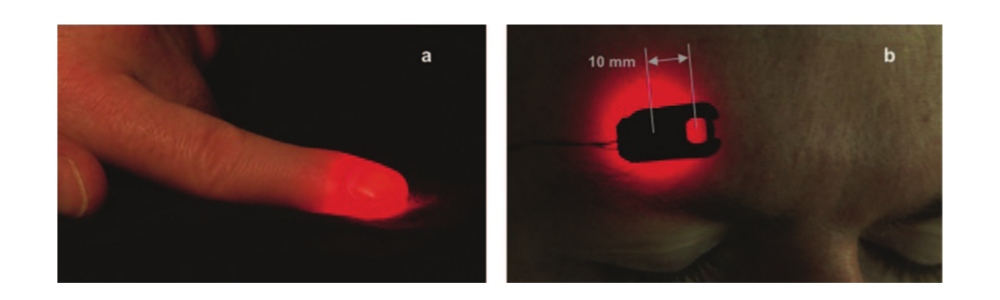
\includegraphics[scale = 0.52]{graphic/redlight.png}}
	\caption{Badanie diagnostyczne przy użyciu światła czerwonego o~długości fali 660 nm metodą transluminacji oraz metodą refleksyjną}
	~\\
	(źródło: Na podstawie \cite{Mann:2007})
	\label{rys:redlight}
\end{figure}

\noindent Natężenie promieniowania wychodzącego z~badanego medium jest wielokrotnie niższe przy zastosowaniu 
metody odbiciowej, gdyż promieniowanie odebrane pochodzi tylko od części promieniowania rozproszonego wstecz. 

\section{Fotopletyzmografia i~pulsoksymetria}
\label{sec:Fotopletyzmografia}

W procesie diagnostyki organizmu żywego ważną rolę odgrywa nieinwazyjne monitorowanie parametrów tętna. Poddając warstwę tkanek promieniowaniu optycznemu, umożliwia się obserwowanie krzywej 
pletyzmograficznej (PPG)~(rys.~\ref{rys:PPG}), której charakterystyczną składową jest fala tętna~\cite{Cys:2007}. Pulsacja krwi tętniczej powoduje niewielkie, cykliczne zmiany objętości 
ośrodka umieszczonego między źródłem a~odbiornikiem. 
\begin{figure}[!ht]
\centerline{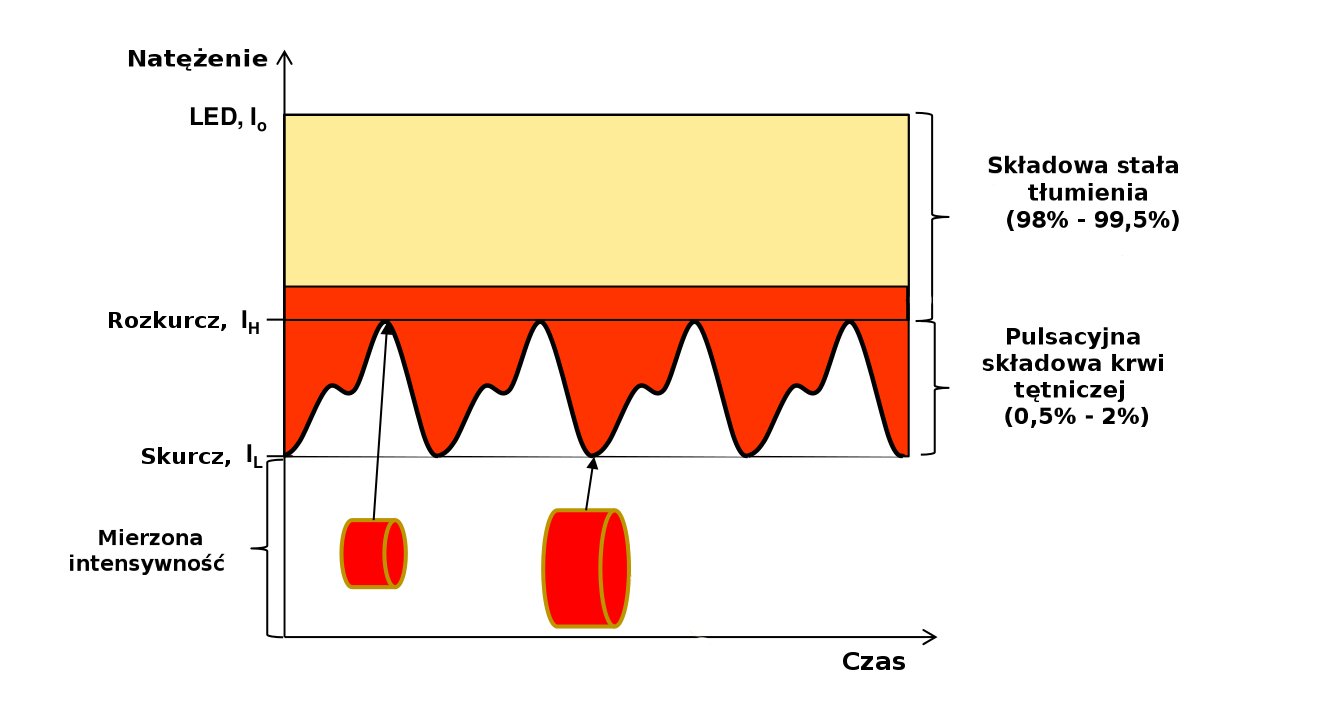
\includegraphics[scale = 0.40]{graphic/PPG.png}}
	\caption{Zmienny przebieg natężenia promieniowania w~następstwie zmian objętości przepływającej krwi w~naczyniach krwionośnych. Wartość natężenia światła osiąga
		 minimum w~chwili przepływu krwi o~najwyższym ciśnieniu}
	~\\
	(źródło: Na podstawie \cite{Dwyer:2008})
	\label{rys:PPG}
\end{figure}
Możliwość detekcji pulsacji tętniczej oraz jej wiarygodne przetworzenie są podstawowym warunkiem realizacji nieinwazyjnego 
optoelektronicznego monitorowania utlenowania krwi tętniczej metodą pulsoksymetrii. W~transmisyjnym wariancie rejestracji sygnałów optycznych występuje, w~porównaniu do wariantu 
odbiciowego, mniejsza wrażliwość na artefakty, niestabilne położenie czujnika oraz inne czynniki zakłócające.

Zgodnie z~zasadami spektrofotometrii, do wykrycia koncentracji $n$ różnych absorberów zawartych w~badanym ośrodku, należy przeprowadzić proces transluminacji dla $n$ różnych długości fali,
przy znanej absorbancji molowej $\alpha(\lambda)$ każdego składnika. Do wykrycia zawartości hemoglobiny ($Hb$) oraz oksyhemoglobiny ($HbO_{2}$) konieczne jest zastosowanie co najmniej
dwóch długości fali, dla których badane substancje wykazują odmienne właściwości optyczne~(rys.~\ref{rys:blood}).
\begin{figure}[ht]
\centerline{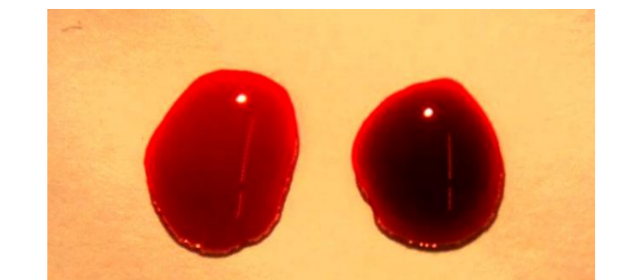
\includegraphics[scale = 0.63]{graphic/blood.png}}
	\caption{Próbki krwi tętniczej oraz krwi żylnej. Różnice w~barwie próbek są skutkiem odmiennych właściwości optycznych hemoglobiny i~oksyhemoglobiny}
	\label{rys:blood}
	~\\
	(źródło: Na podstawie \cite{Dwyer:2008})
\end{figure}

W~celu najgłebszej penetracji promieniowania świetlnego, podczas określania saturacji krwi stosuje się źródła światła o~długościach fali 660~nm oraz 940~nm zawarte w~oknie optycznym tkanek żywych 
(rys.~\ref{rys:RIR}). Fotodetektor stanowi zazwyczaj pojedyncza krzemowa dioda PIN, generująca prąd fotoelektryczny o~wartości proporcjonalnej do natężenia przepuszczonego promieniowania świetlnego. 

Ponieważ częstość zmian objętości naczyń krwionośnych odpowiada częstości skurczów serca, krzywa pletyzmograficzna może być wykorzystana do łatwego wyznaczania tętna. Właściwa częstość 
akcji serca jest równa liczbie globalnych punktów ekstremalnych krzywej PPG w~określonym przedziale czasu.
\begin{figure}[h]
\centerline{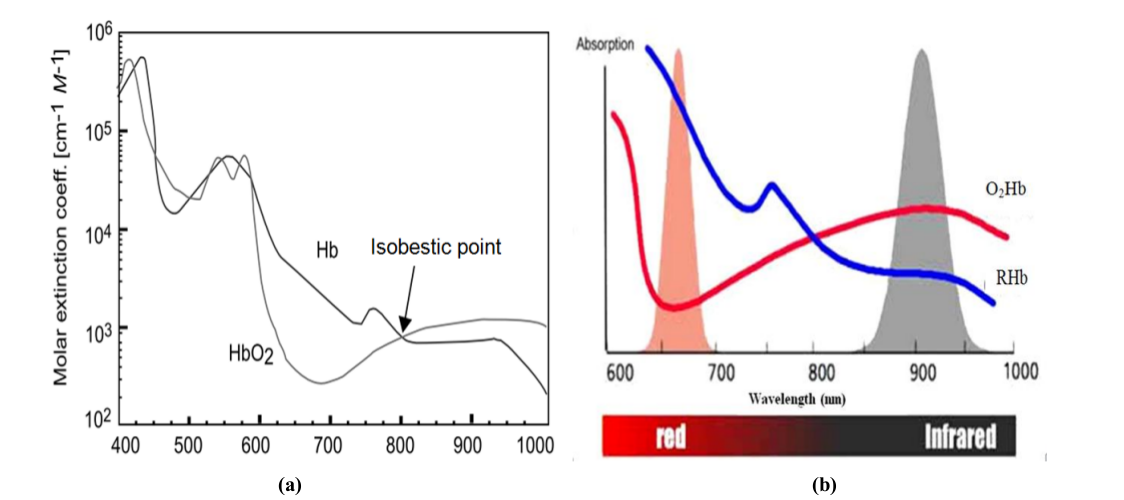
\includegraphics[scale = 0.46]{graphic/RIR.png}}
	\caption{Fragment widma absorpcyjnego hemoglobiny i~oksyhemoglobiny}
	\label{rys:RIR}
	~\\
	(źródło: Na podstawie \cite{Dwyer:2008})
\end{figure}

Pomiar saturacji częściowej $SpO_{2}$ to operacja złożona w~stosunku do pomiaru częstości akcji serca. Natężenie promieniowania odbieranego przy podświetlaniu obiektu złożonego z~tkanek
żywych nie jest wartością stałą w~czasie. Skutkiem istnienia podskórnych naczyń krwionośnych w~postaci tętnic i~żył, krzywa pletyzmograficzna składa się z~dwóch składowych: stałej (DC) oraz zmiennej 
(AC)~(rys.~\ref{rys:maxmin2}). Składowa stała stanowi część promieniowania świetlnego transmitowaną przez warstwę tkanek stałych nie zmieniających znacząco swojej objętości w~przedziale czasu jak: 
kości, skóra, mięśnie, tkanka tłuszczowa~\cite{Fuzzy:2011}.
\begin{figure}[!h]
\centerline{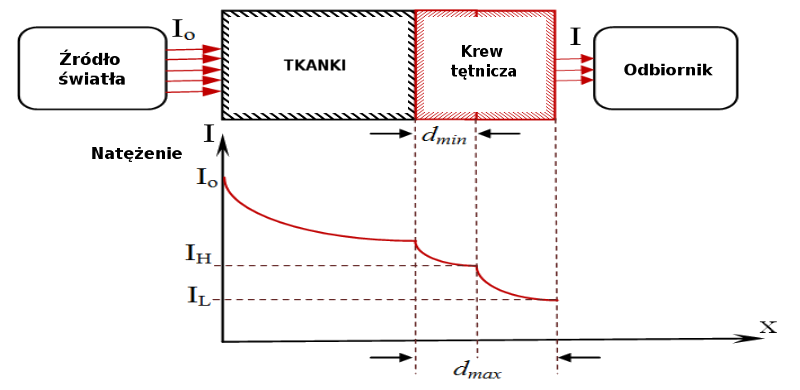
\includegraphics[scale = 0.50]{graphic/maxmin2.png}}
	\caption{Interpretacja wartości minimalnej oraz maksymalnej natężenia promieniowania na podstawie równania Lamberta-Beera}
	\label{rys:maxmin2}
	~\\
	(źródło: Na podstawie \cite{Dwyer:2008})
\end{figure}

W~celu wyznaczenia natężenia promieniowania metodą transluminacji w~tkankach żywych, stosowane jest prawo Lamberta-Beera dla środowiska~niehomogenicznego~(\ref{equ:equ1}).
\begin{equation}
\label{equ:equ1}
	I(t)=I_{0}e^{-(\alpha_{DC}C_{DC}d_{DC}+(\alpha_{Hb}C_{Hb}+\alpha_{HbO_{2}}C_{HbO_{2}})d(t))}
\end{equation}
gdzie:\\
$\alpha_{DC}C_{DC}d_{DC}$ - składowa stała tłumienia tkanek żywych,\\
$\alpha_{Hb}, \alpha_{HbO_{2}}$ - molowy współczynnik absorpcji hemoglobiny i~oksyhemoglobiny,
$C_{Hb}, C_{HbO_{2}}$ - stężenie molowe hemoglobiny i~oksyhemoglobiny.\\

%\noindent Czynnik $(\alpha_{Hb}C_{Hb}+\alpha_{HbO_{2}}C_{HbO_{2}})d(t)$ stanowi składową pulsacyjną  tłumienia. 
\noindent Wartość maksymalna $I_{H}$ oraz minimalna $I_{L}$ natężenia promieniowania odebranego~(rys.~\ref{rys:maxmin1}) wynoszą odpowiednio:
 
\begin{equation}
\label{equ:equ2}
	I_{H}=I_{0}e^{-(\alpha_{DC}C_{DC}d_{DC}+(\alpha_{Hb}C_{Hb}+\alpha_{HbO_{2}}C_{HbO_{2}})d_{H})}
\end{equation}

\begin{equation}
\label{equ:equ3}
	I_{L}=I_{0}e^{-(\alpha_{DC}C_{DC}d_{DC}+(\alpha_{Hb}C_{Hb}+\alpha_{HbO_{2}}C_{HbO_{2}})d_{L})}
\end{equation}
\noindent W~celu uproszczenia i~wyeliminowania funkcji wykładniczej z~równań~(\ref{equ:equ2}) oraz~(\ref{equ:equ3}) obliczamy logarytm naturalny z~ilorazu $I_{H}$ i~$I_{L}$ otrzymując:

\begin{equation}
\label{equ:equ4}
	ln(\frac{I_{H}}{I_{L}})=(\alpha_{Hb}C_{Hb}+\alpha_{HbO_{2}}C_{HbO_{2}})\Delta d
\end{equation}
gdzie:\\
$\Delta d=d_{H}-d_{L}$

\begin{figure}[ht]
\centerline{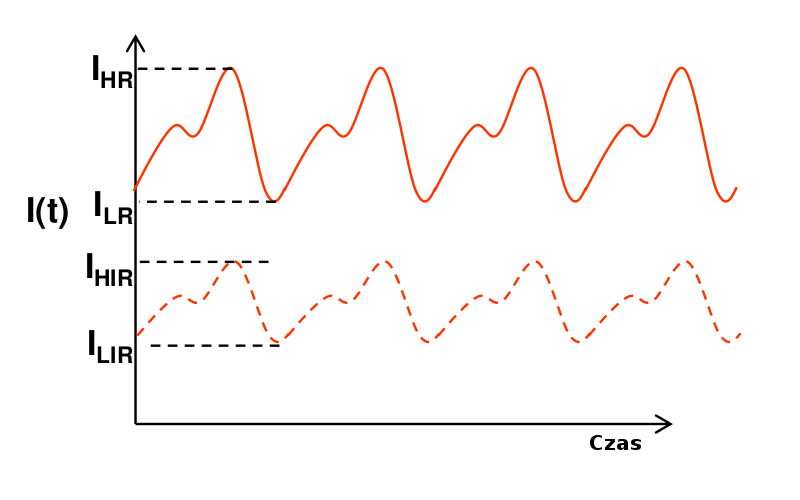
\includegraphics[scale = 0.40]{graphic/maxmin1.png}}
	\caption{Krzywa pletyzmograficzna (PPG) badanego ośrodka dla 660~nm oraz 940~nm}
	\label{rys:maxmin1}
	~\\
	(źródło: Na podstawie \cite{Dwyer:2008})
\end{figure}

\noindent Dla obu długości fali 660~nm oraz 940~nm otrzymano dwa równania z~dwoma niewiadomymi $C_{Hb}$ i~$C_{HbO_{2}}$. Iloraz obu równań oznaczono jako współczynnik~$R$:

\begin{equation}
\label{equ:equ4}
	R=\frac{ln(\frac{I_{HR}}{I_{LR}})}{ln(\frac{I_{HIR}}{I_{LIR}})}=\frac{\alpha_{Hb}(\lambda_{R})C_{Hb}+\alpha_{HbO_{2}}(\lambda_{R})C_{HbO_{2}}}{\alpha_{Hb}C(\lambda_{IR})_{Hb}+\alpha_{HbO_{2}}(\lambda_{IR})C_{HbO_{2}}}
\end{equation}\\
\noindent Przy założeniu, że $\Delta d_{R} = \Delta d_{IR}$.\\ 
\noindent Następnie wyznaczono zawartość procentową hemoglobiny utlenowanej w~całkowitej ilości hemoglobiny~\cite{Fuzzy:2011}.

\begin{equation}
\label{equ:equ4}
	SpO_{2}=\frac{C_{Hb}}{C_{Hb}+C_{HbO_{2}}}~100\%
\end{equation}

\begin{equation}
\label{equ:equ5}
	SpO_{2}=\frac{\alpha_{Hb}(\lambda_{R})-\alpha_{Hb}(\lambda_{IR})R}{\alpha_{Hb}(\lambda_{R})-\alpha_{HbO_{2}}(\lambda_{R})+(\alpha_{Hb}(\lambda_{IR})-\alpha_{HbO_{2}}(\lambda_{IR}))R}~100\%
\end{equation}

\noindent Wyznaczenie teoretycznej wartości wysycenia krwi tętniczej ograniczone zostało do obliczenia parametru $R$~zależnego od wartości maksymalnej i~minimalnej natężenia 
odebranego promieniowania dla obu długości fali~(rys.~\ref{rys:saturation}).

Aproksymacja prawa Lamberta-Beera, eliminująca składową rozpraszania i~odbicia promieniowania na wartość tłumienia ośrodka~(\ref{equ:equ1}), wprowadza błąd pomiarowy w~procesie wyznaczania wysycenia krwi 
tlenem~\cite{Web:1997}. Obliczenia dokonane zostały przy założeniu, że natężenie padającego promieniowania jest sumą natężenia odebranego oraz promieniowania tłumionego w~ośrodku. W~normalnych
warunkach pracy pulsoksymetru, zmierzona wartość nasycenia jest wystarczająca do celów klinicznych, pomimo pominięcia znaczącego tłumienia światła pod wpływem rozpraszania. 

Większość komercyjnych urządzeń do pomiaru wskaźnika $SpO_{2}$ wykorzystuje empiryczną zależność wysycenia krwi od parametru $R$~(rys.\ref{rys:saturation}), wyznaczoną poprzez chemiczną analizę 
składu krwi (in~vitro). Proces kalibracji aparatu pomiarowego eliminuje błędy wprowadzane na skutek uproszczeń dokonanych podczas wyprowadzania teoretycznych zależności.
\begin{figure}[ht]
\centerline{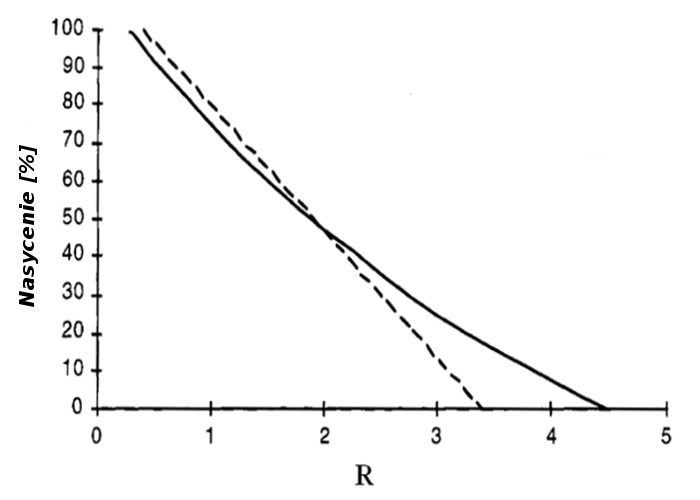
\includegraphics[scale = 0.52]{graphic/saturation.png}}
	\caption{Teoretyczna (linia ciągła) i~empiryczna (linia przerywana) krzywa zależności wskaźnika wysycenia krwi tętniczej tlenem w~funkcji parametru~$R$}
	\label{rys:saturation}
	~\\
	(źródło: Na podstawie \cite{Dwyer:2008})
\end{figure}

\section{Uwarunkowania i~ograniczenia pomiarowe}
\label{sec:Ograniczenia}

Urządzenia monitorujące nasycenie krwi są standardem na oddziałach intensywnej terapii, których niezawodna praca pozwala na właściwą ocenę stanu pacjenta. W~celu uzyskania optymalnej wydajności
i~precyzji, należy wyeliminować czynniki zaburzające warunki przeprowadzanego pomiaru. 

\subsubsection{Ograniczenia fizjologiczne}
\label{subsubsec:fizj}

Wartość wysycenia $SpO2$ jest fizjologicznie związana z~ciśnieniem parcjalnym $PaO2$~\cite{Fuzzy:2011}. Zależność saturacji krwi od wartości $PaO2$ przedstawia rysunek~(rys.\ref{rys:PaO2}).
Wysokim wartościom współczynnika $SpO2$ odpowiadają niewielkie zmiany ciśnienia parcjalnego tlenu. W~zakresie ciśnienia 0-80~mmHg, niewielkie zmiany ciśnienia powodują znaczące wahania
współczynnika saturacji $SpO2$.
\begin{figure}[ht]
\centerline{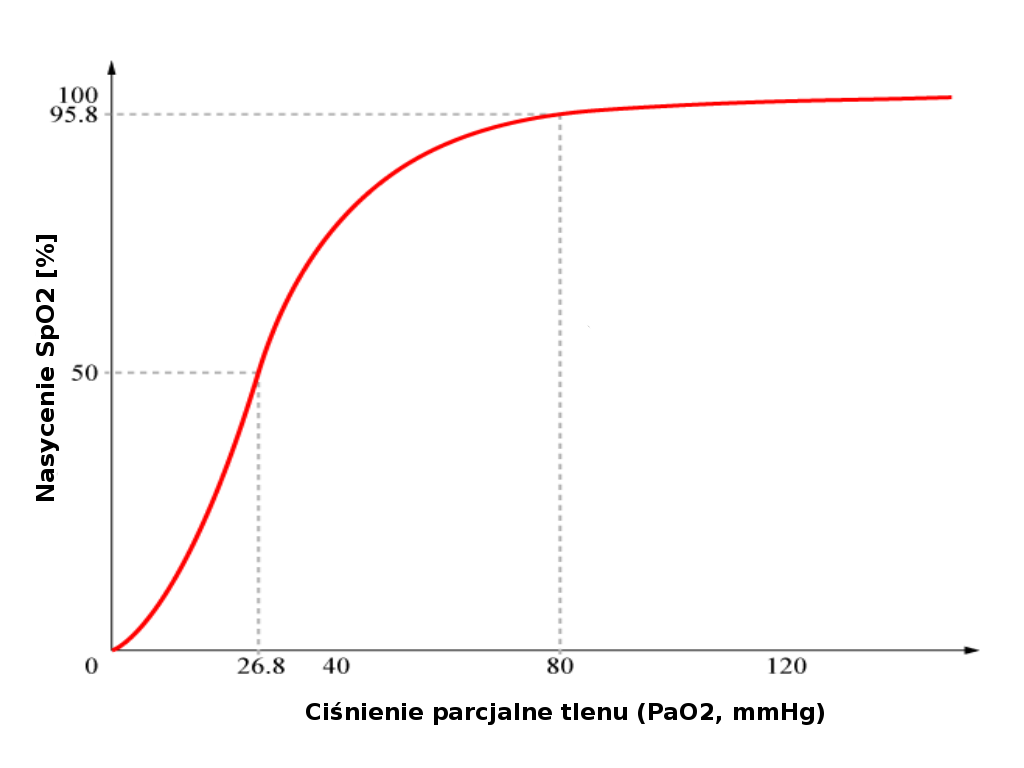
\includegraphics[scale = 0.32]{graphic/PaO2}}
	\caption{Krzywa dysocjacji oksyhemoglobiny. Zależność wysycenia krwi tlenem od ciśnienia parcjalnego $PaO2$}
	\label{rys:PaO2}
	~\\
	(źródło: Na podstawie \cite{Fuzzy:2011})
\end{figure}

Zastosowanie dwóch długości fali w~pomiarach wskaźnika nasycenia krwi, umożliwia określenie stężenia tylko dwóch substancji o~odmiennych właściwościach optycznych. Występowanie związków
hemoglobiny z~tlenkiem węgla, siarką oraz hemoglobiny dysfunkcyjnej powoduje zaburzanie wyniku pomiarów.
Pigmentacja skóry oraz inne absorbery, jak np.~płytka paznokcia, skutecznie tłumią wiązkę promieniowania transmitowanego, co często uniemożliwia uzyskanie odpowiednio silnego sygnału w~odbiorniku.

Płaski kształt czerwonych krwinek powoduje zmianę powierzchni pochłaniania promieniowania podczas skurczu oraz rozkurczu serca~\cite{Fuzzy:2011}. W~chwili skurczu, gdy w~naczyniach 
krwionośnych panuje najwyższe ciśnienie, erytrocyty pod wpływem strumienia przepływającej krwi, ustawiają się prostopadle do kierunku przepływu, zmniejszając aktywną powierzchnię 
absorbującą~(rys.\ref{rys:sysdias}).

\begin{figure}[ht]
\centerline{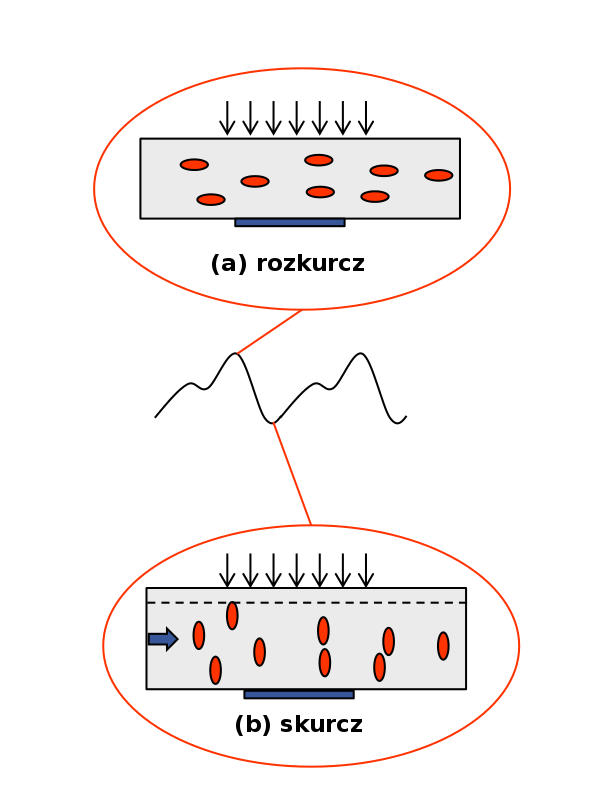
\includegraphics[scale = 0.40]{graphic/sysdias}}
	\caption{Ułożenie krwinek czerwonych podczas skurczu i~rozkurczu serca}
	\label{rys:sysdias}
	~\\
	(źródło: Na podstawie \cite{Fuzzy:2011})
\end{figure}

\subsubsection{Ograniczenia związane z przetwarzaniem sygnałów}
\label{subsubsec:fizj}

Najpoważniejszym zagrożeniem podczas przetwarzania sygnałów dostarczonych z~detektora promieniowania są zakłócenia spowodowane ruchem mierzonego obiektu umieszczonego
w~klipsie pulsoksymetru~(rys.\ref{rys:noise}). Użyteczny sygnał zawierający pulsującą składową tętna jest wielokrotnie słabszy od powstających zakłóceń. W~celu uniknięcia
zniekształceń sygnału użytecznego, pomiar saturacji krwi powinien przebiegać przy całkowitym unieruchomieniu kończyny, na której znajduje się klips pomiarowy.

\begin{figure}[ht]
\centerline{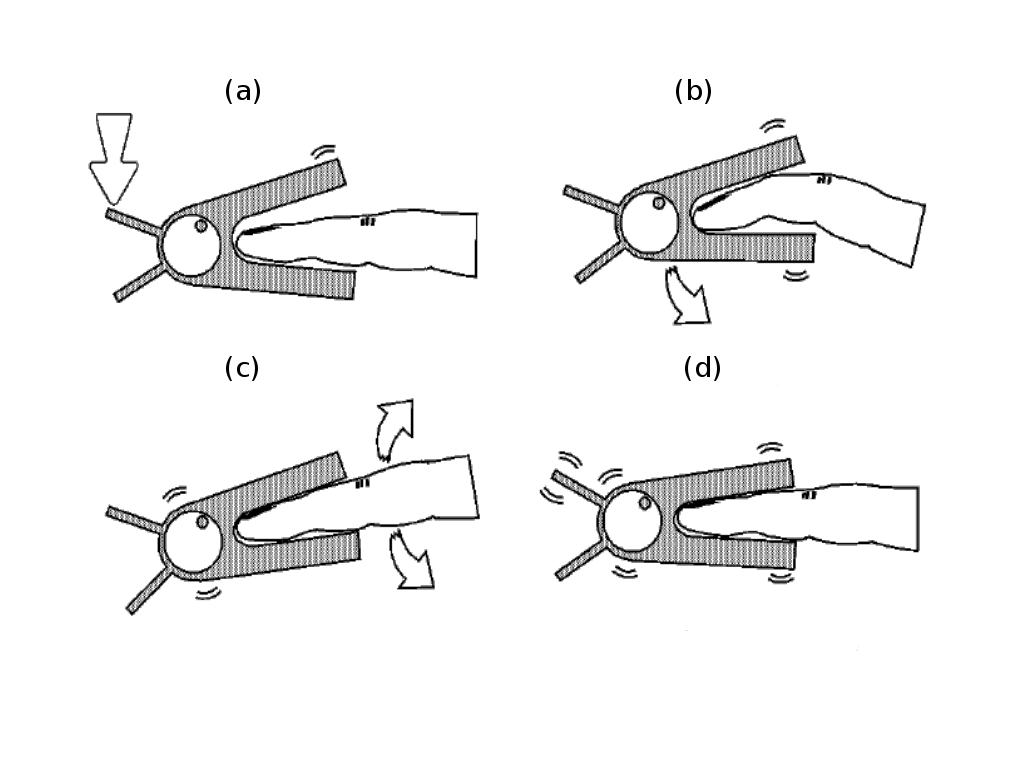
\includegraphics[scale = 0.38]{graphic/noise}}
	\caption{Przykłady nieprawidłowego umieszczenia palca w~klipsie pomiarowym: nieprawidłowe dociśnięcie klipsa~(a), zginanie obiektu~(b), poruszanie obiektu wraz z~klipsem~(c)
		oraz drgania obiektu wraz z~klipsem~(d)}
	\label{rys:noise}
	~\\
	(źródło: Na podstawie \cite{Dwyer:2008})
\end{figure}

Przedstawiona metodyka pomiaru wysycenia krwi została opracowana przy założeniu, że składowa pulsacyjna krzywej pletyzmograficznej jest związana tylko i~wyłącznie z~przepływem krwi tętniczej.
W~rzeczywistości, powracająca krew żylna wprowadza dodatkową składową zmienną o~niewielkiej amplitudzie~(rys.\ref{rys:vein}). Sposób wyznaczania saturacji $SpO2$ opiera się na analizie amplitudowej 
sygnału zmiennego, otrzymanego w~procesie transluminacji. Skutkiem występowania składowej zmiennej odtlenowanej krwi żylnej (saturacja 65\%~-~75\%) jest wprowadzenie błędu pomiarowego w~procesie 
wyznaczania prawidłowego współczynnika wysycenia krwi tętniczej~\cite{Fuzzy:2011}. 

\begin{figure}[h]
\centerline{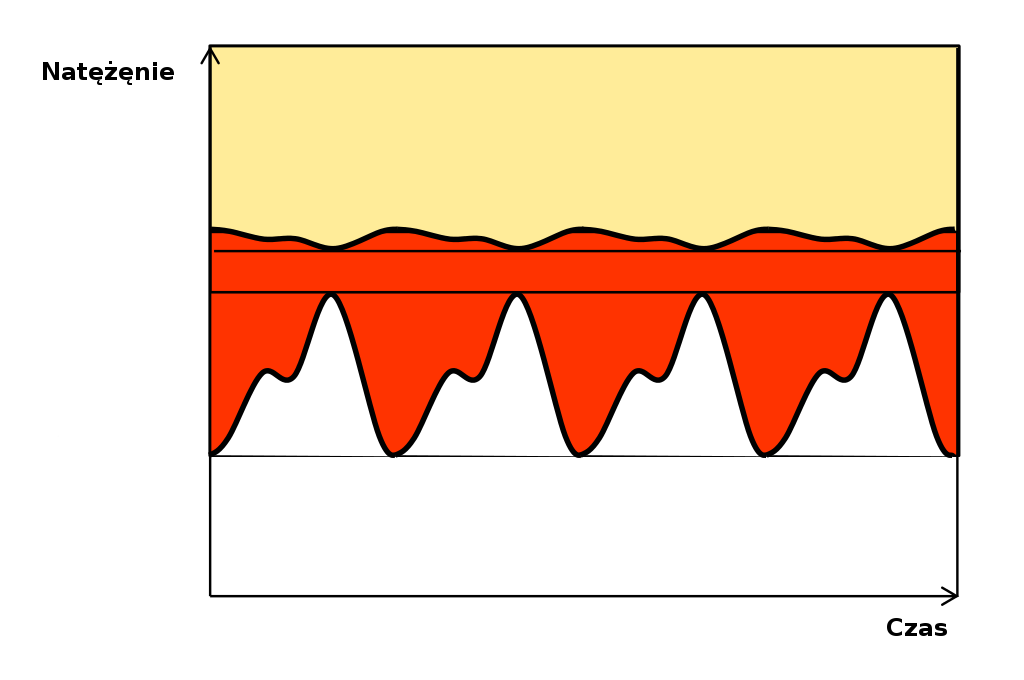
\includegraphics[scale = 0.36]{graphic/vein}}
	\caption{Krzywa pletyzmograficzna (PPG) krwi tętniczej wraz ze składową zmienną krwi żylnej}
		
	\label{rys:vein}
	~\\
	(źródło: Na podstawie \cite{Dwyer:2008})
\end{figure}

Poważnym problemem pomiarowym jest wpływ obcego promieniowania występującego w~sąsiedztwie stanowiska pomiarowego. W~przeciwieństwie do natężenia promieniowania stałego w~czasie, najpoważniejszym 
problemem jest promieniowanie pochodzące od źródeł światła zasilanych bezpośrednio z~sieci~energetycznej. 
Pojawienie się składowej zmiennej o~częstotliwości 50~-~60~Hz w~sąsiedztwie widma częstotliwościowego sygnału użytecznego, narzuca konieczność stosowania filtrów dolnoprzepustowych o~stromych zboczach 
w~celu uniknięcia degradacji~sygnału użytecznego.

